\section{Analysis of Motor Data}
\label{sec:analysis}

\subsection{Motor components and setup}

A basic DC motor consists of a stator, a rotor, a commutator, an external magnetic field, brushes, bearings and a shaft. A DC power supply is connected across the brushes, transmitting power through the commutator into windings around the rotor. The current flowing through the windings interacts with the permanent magnetic field producing a Lorentz force, seen in Equation~\eqref{Lorentz} resulting in a torque across the windings.
%reference lorentz
\begin{equation}
    F = I L \times B
    \label{Lorentz}
\end{equation}

As the rotor spins away from a position with the windings perpendicular to the magnetic field, the torque is reduced. To allow a rotational force over the full revolution, commutators invert the current flow periodically. 

\begin{figure}
    \centering
    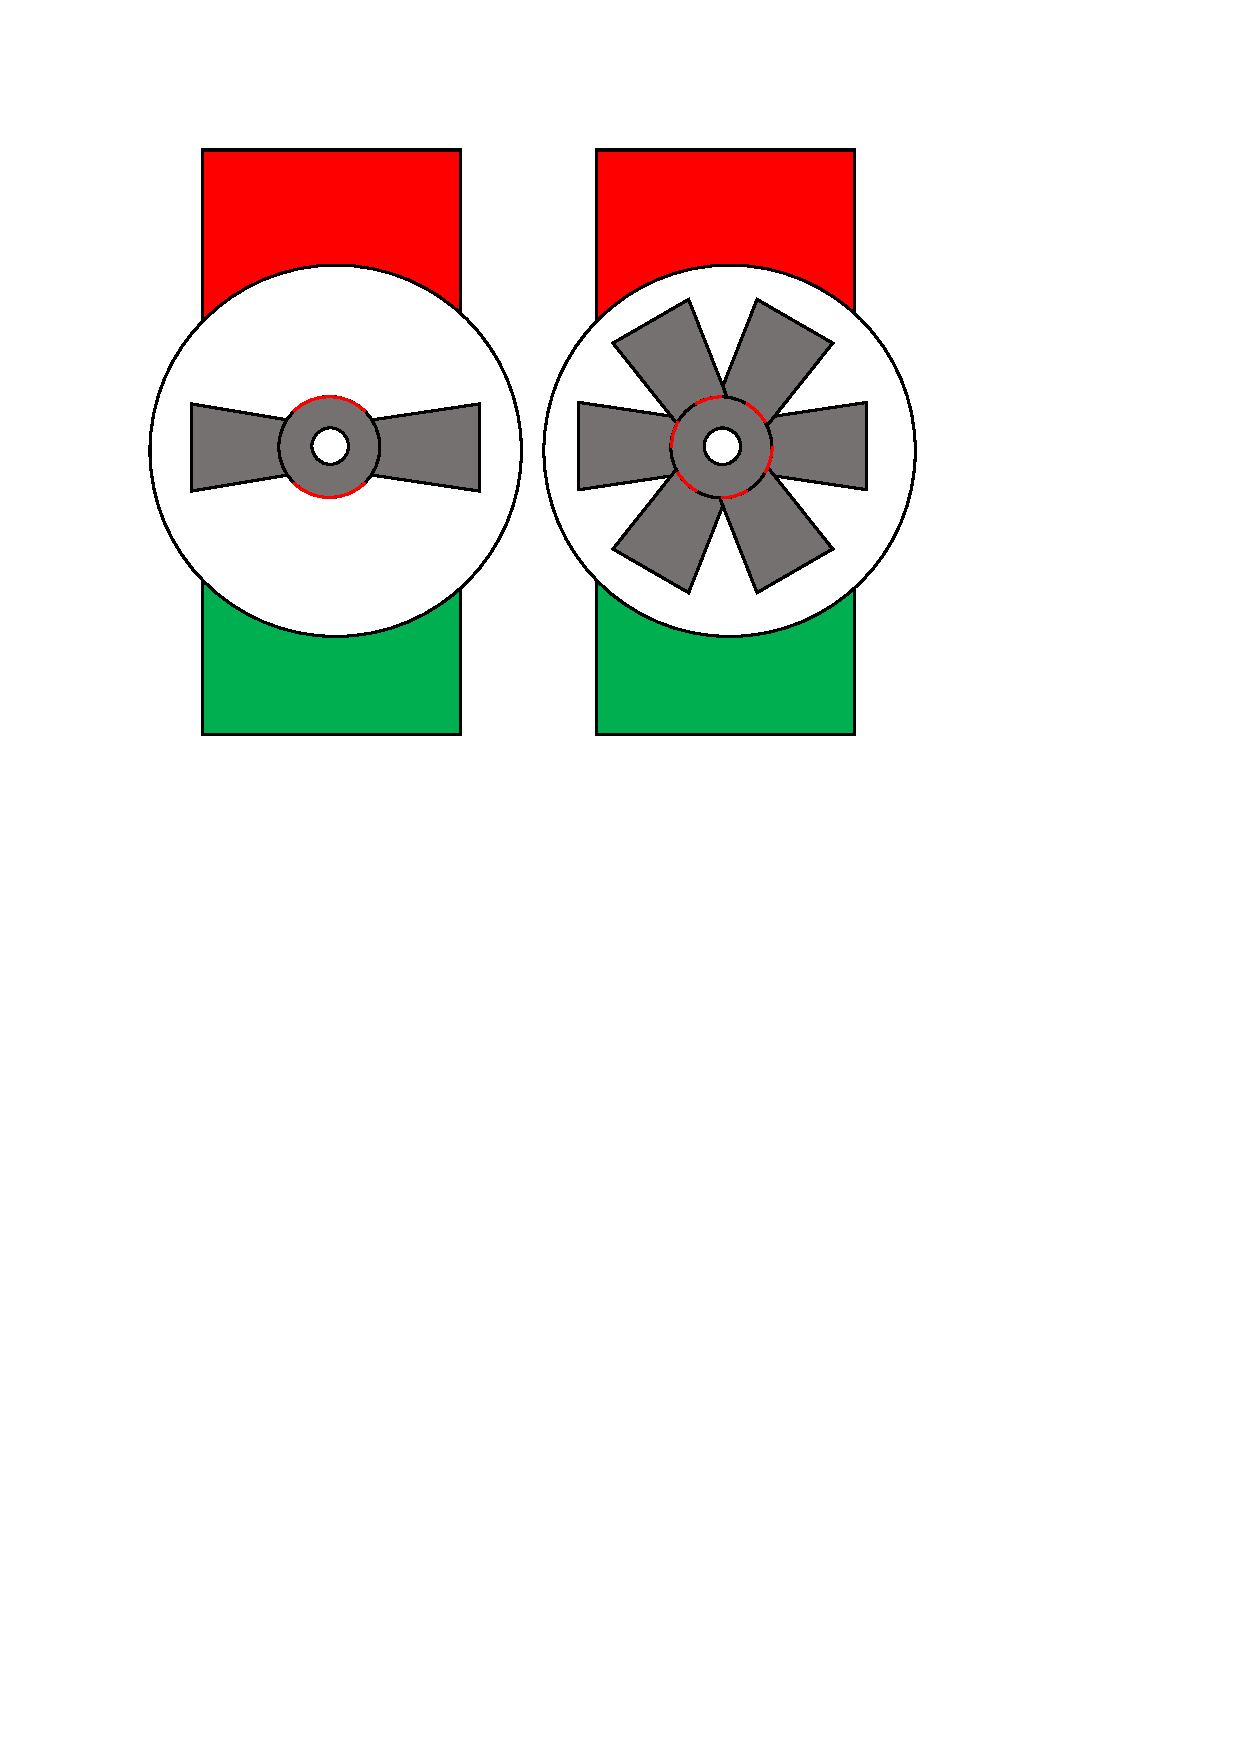
\includegraphics[trim={2cm 15.5cm 0cm 2.548cm}, clip, width=0.8\textwidth]{2polevs6polemotor.pdf}
    \caption[DC motor cross sectional comparison]{This shows a cross sectional comparison between a two pole and six pole motor at various rotation stages. The top left image is labelled showing the: 1. Axle, 2. Commutator, 3. Rotor with windings, 4. Permanent magnets, 5. Stator.}
    \label{fig:2pole_vs_6pole}
\end{figure}

In the simplest possible motor, the rotor is composed of only one set of windings, with a split ring commutator inverting the power supply every half rotation. A more efficient model is to have multiple windings that receive power throughout different stages in the rotation shown in Figure.~\ref{fig:2pole_vs_6pole}. 

At the beginning of the cycle of the two pole motor, the permanent magnetic field is perpendicular to the windings, giving a maximum torque. After one quarter rotation, the windings are parallel to the field. This provides no torque and there is a momentary loss in power as the current is inverted by the commutator. The motor continues to spin due to the momentum gained in the initial stage of rotation until the current is inverted, when torque is regained. For the six pole motor, there is initially a maximum torque supplied by the red marked windings, which decreases to zero at the quarter rotation stage. Unlike the two pole motor, this loss of torque is compensated for, by an increase in torque of the two yellow windings. The torque provided here is more constant than the simple two pole motor, however still not perfectly continuous. An increase in the number of poles increases the continuity of rotation.

The brushes of a motor can be either spring loaded carbon rods, or copper strips pressed against the commutator. Carbon rods are far more efficient and less damaging to the motor, the reasons for this will be discussed further. With advancements in technology, brushless DC motors are becoming increasingly popular, removing the inefficiencies induced by the traditional brushes. 

Mechanical components, such as the bearings, shaft or motor housing are prone to physical damage. This could be due to either physical trauma or a contamination within the motor during operation. Failure of this type would need heavy repairs, with sometimes expensive replacements necessary, it is therefore important to diagnose any unhealthy running motor to minimise the damage.

\begin{figure}
    \centering
    \begin{circuitikz} 
    \draw (0.9,0.75) node[left] {5 V};
    \draw (5.5,0) node[left] {2};
    \draw (5.5,1) node[left] {1};
    \draw (5.5,-1) node[left] {3};
    \draw (10.5,0) node[left] {V$_2$ out};
    \draw (10.5,1) node[left] {V$_1$ out};
    \draw (10.5,-1) node[left] {V$_3$ out};
    \draw
    (0,0) to[battery]  (1,0)
          to[generic]  (9,0) -- (9,0)
          to[short,-o] (9,0)
    ;
    \draw
    (2,0) to[ground] (2,1)
          to[generic] (8,1) -- (8,1)
              to[short,-o] (9,1)
    ;
    \draw
    (2,0) to[ground] (2,-1)
          to[generic] (8,-1) -- (8,-1)
          to[short,-o] (9,-1)
    ;
    \draw
    (8,1) to[short] node[ground] {} (8,-3)
    ;
    \end{circuitikz}
    \caption[Sensor circuit board]{The circuit required to convert data recorded by the contact microphones from an anologue output to digital so that it can accessed by the National instruments DAQ box.}
    \label{fig:circuit_diagram}
\end{figure}

The vibrational data collected by the contact microphones provided an analogue output, which when passed through a NI multifunction DAQ\footnote{NI USB-6009  Multifunction DAQ USB Device, Datasheet: \url{http://www.ni.com/datasheet/pdf/en/ds-218}}, could be converted and saved as a csv file. The circuit diagram showing the configuration of components is displayed in Figure.~\ref{fig:circuit_diagram}. This was produced using a Veroboard.

The rotation speed of a motors shaft can provide a lot of information about the running health of a motor. Measurements of rotation speed can be obtained through the use of a rotary encoder (footnote style thing here) (maybe picture here? Take on Wednesday) which is fitted to the rotating shaft. The encoder is a composed of a codewheel and an emitter/detector module. As the disk spins, the apertures periodically block or allow the light to pass from the emitter to detector, converting the rotary shaft motion into a digital output. The rotary disk has three sections for varying level of accuracy, one channel outputs once per revolution, the other providing higher resolution with COUNT ROTARY ENCODER SLITS.

The quadrature output of the rotary encoder allows monitoring of the shaft rotation speed with time, allowing investigation into certain failure modes such as slipping. This piece of equipment is relatively invasive compared to the contact microphones, as it requires fixing to the shaft, limiting space for operational output. 


\subsection{Calibration Tests}

In order to determine which frequency components were from the motors and what was simply noise (unwanted signal), calibration tests were run for each motor. This involved recording data whilst the motor was off. 

\begin{figure}[t]
    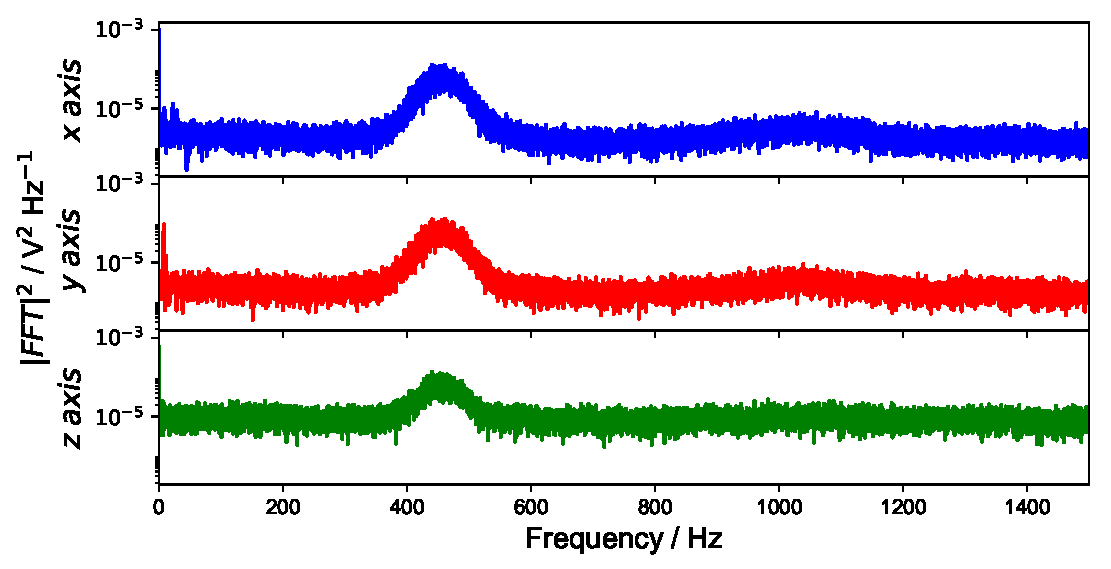
\includegraphics[width=1.0\textwidth]{fig/freq_large_0V.pdf}
    \caption[Calibration Frequency 1]{The Fourier spectra in the x, y, and z axes for the large motor at 0V.}
    \label{fig:freq_large0V}
\end{figure}

Figure~\ref{fig:freq_large0V} shows the frequency spectra for a calibration test with the large motor. 

----write more

\subsection{Baseline Tests}

\begin{figure}[t]
    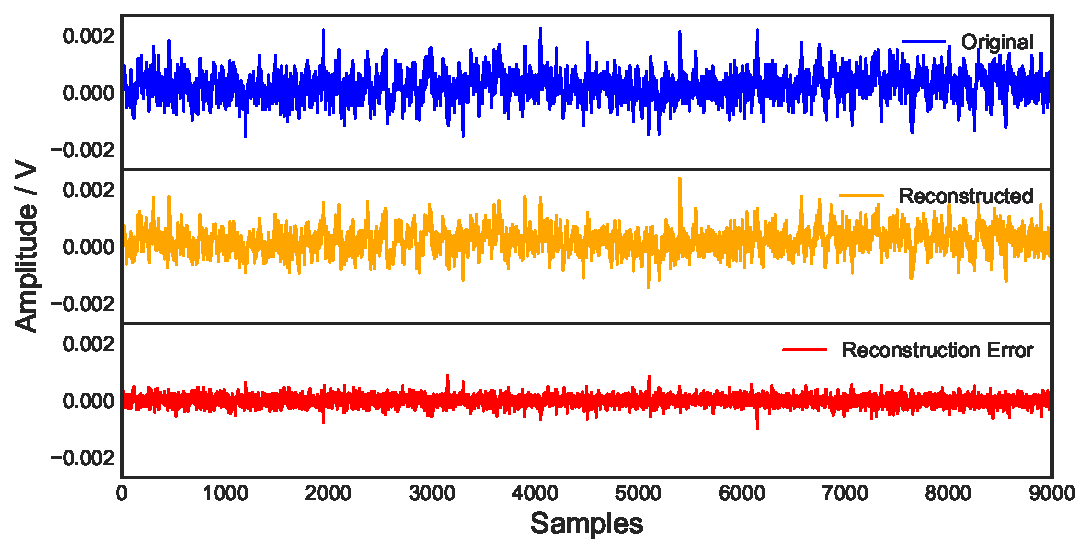
\includegraphics[width=1.0\textwidth]{fig/kmeans_large_4Vnowater.pdf}
    \caption[K-means Large Motor Reconstruction No Water]{K-means reconstruction applied to three seconds of data from large motor running at 4 V. Top: the original testing data. Middle: the reconstruction using K-means. Bottom: the reconstruction error between the reconstructed and original signal.}
    \label{fig:kmeans_large4V}
\end{figure}

Figure.~\ref{fig:kmeans_large4V} shows the K-means reconstruction of a three second signal using training and testing data both from a baseline test run. The first three seconds of the baseline test run was used as training data and the second three seconds used as fitting data. This was done to check if the synthetic segments could be used to recreate a later section of the same baseline run with minimal reconstruction error. 

\subsection{Overheating}
%talk about snipped coils too to simulate each coil breaking separetly.

Overheating is widely regarded as the most common cause of motor failures, with many other types of motor deterioration leading to overheating. This is such a substantial problem that a rise of just 10 $^o$C above the regular running temperature causes the life expectancy of the motor to halve. The life span is halved once again for every 10 $^o$C the temperature is raised further.

The problem arises as, during overheating, the varnish covering the metal wires begins to melt. If this occurs at two points of wires that are in contact, the coil of the motor can short circuit.

%(Gears Removed motor)

In order to induce motor failure, a motor, shown in Figure.~\ref{fig:hotplate_motor}, consisting of 7 coils separately providing power was placed on a hotplate, heated to 150 $^o$C, for one hour. This was compared to the assumed usual running temperature of 60 $^o$C, meaning that just one hour on the hot plate equated to 512 hours of regular use.

For this failure mode, only coil was in direct contact with the plate so as only to damage that coil, leaving the others, ideally, with little impairment. Despite the fact that some heat would obviously be conducted through the motor, the effect of this was considered to be minimal with respect to the effect on the targeted coil.

The result of just one coil being broken is that there would be a brief loss of power in the motor when this coil was in contact with the brushes. Therefore the speed of revolution would no longer be uniform. This can cause other problems to occur in the motor such as damage to the bearings. 

In case this did not result in the targeted coil breaking entirely, a further experiment was devised that simulated this effect. To inhibit just one coil, one of the coils was cut. It was then observed that the rotation speed was not constant with no power being given to the motor for $({2}/{7})$ of the time - due to the fact that either of the two brushes could be in contact with the broken coil. Further coils were cut and the speed noted to become even more erratic until. Once four had been broken, the motor was unable to run at all as there was never a point where two brushes were in contact with working coils.

\begin{figure}[t]
    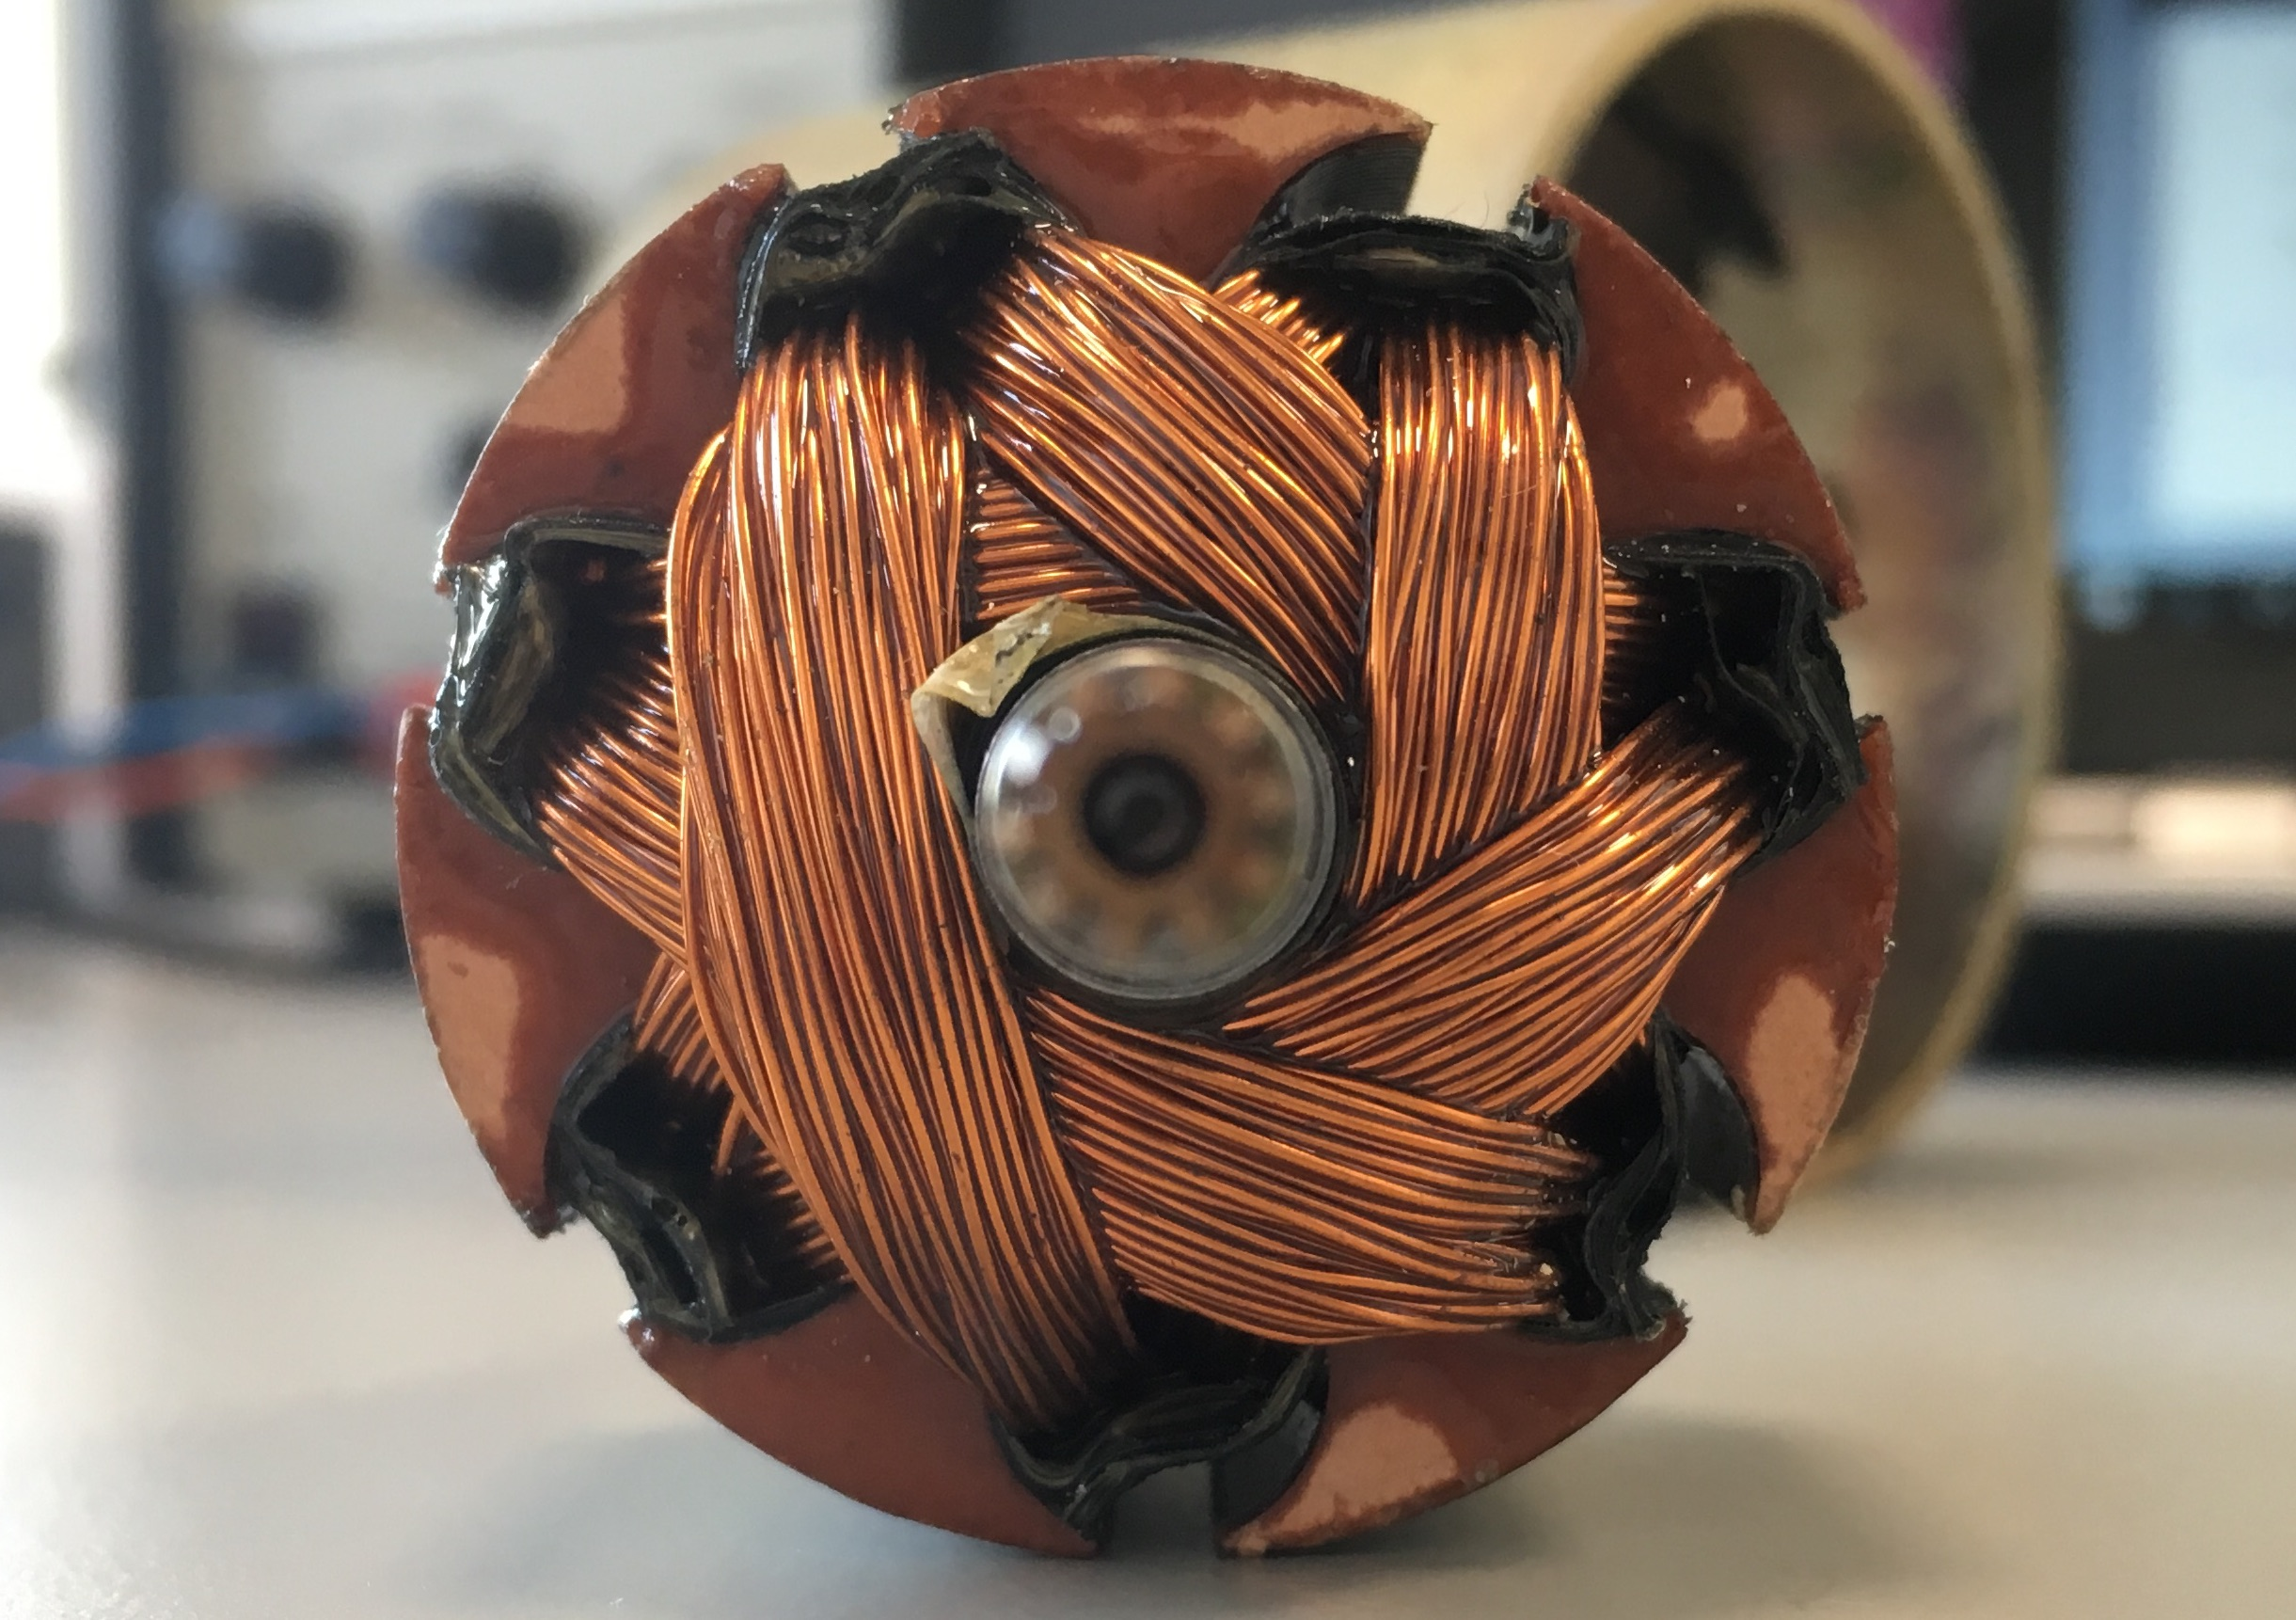
\includegraphics[width=1.0\textwidth]{fig/Gears_Removed_Inside.JPG}
    \caption[Motor Placed on Hotplate]{The inside of the Gears removed motor showing the 7 separate coils, one of which was placed directly on the hotplate at 150 $^o$C for one hour to induce failure.}
    \label{fig:hotplate_motor}
\end{figure}

In addition to this, the motor was placed in an oven at 200 $^o$C for 2 hours to cause extensive damage to all the coils evenly. This equates to over 30,000 hours of running in regular conditions. This was considered sufficient to bring the motor very close to failure given the typical life span of a 12 V motor is just 1000 hours. %1000???
Data was then collected for one minute to find any lasting damage.

%Need references from papers for this


\subsection{Overvoltage}

An increase in voltage will also cause an increase in current, resulting in more eddy currents in the wires and subsequently heating the motor. As stated earlier, this is a major reason for motor failures. 

Moreover, overvoltaging causes the torque of the motor to increase. The subsequent increased rotation speed leads to the rotor slipping. In order to reduce this slip, the motor will then draw an even greater current further contributing to the overheating effect. As well as this, a greater rotation speed will increase friction and will wear down bearings and brushes. Just a small increase in voltage can result in a large amount of damage as,

\begin{equation}
\tau \propto V^2,
\label{Torque}
\end{equation}

where $\tau$ is torque and $V$ is voltage.

In addition to the detrimental effect of overvoltaging, undervoltaging can be just as destructive. In fact, the effect of slipping is even more prominent when a motor is not given enough power and leads to more overheating.

%12V motor

The effect of overvoltaging  was investigated by running a 12 V motor at increasingly high voltages ranging from 12 V to 30 V. This was done for just one minute each time and was used to find the immediate effects of overvoltaging a motor.
    
%Large Motor

A second motor, also with a regular operating voltage of 12 V, was run at 30 V for one hour. In this instance, the bearings reached 90 $^o$C; this demonstrates the extreme effects of overvoltaging a motor. Readings could not be taken during this run as the sensors are only able to operate %Need synonym
up to 60 $^o$C. %Correct???
Therefore, readings were taken before and after the one hour run. This allowed us to explore the long term effects of overvoltaging a motor.

%Undervoltage experiment (large motor)

In order to investigate the effects of undervoltaging a motor, data was collected when running a 12 V motor from 1 V through to 5 V, in 1 V instalments. The speed of rotation could be seen to be irregular, providing evidence that the rotor was slipping. This speed was taken using the rotary encoder, mentioned earlier.

%Again need references.

\subsection{Load}

\begin{figure}[t]
    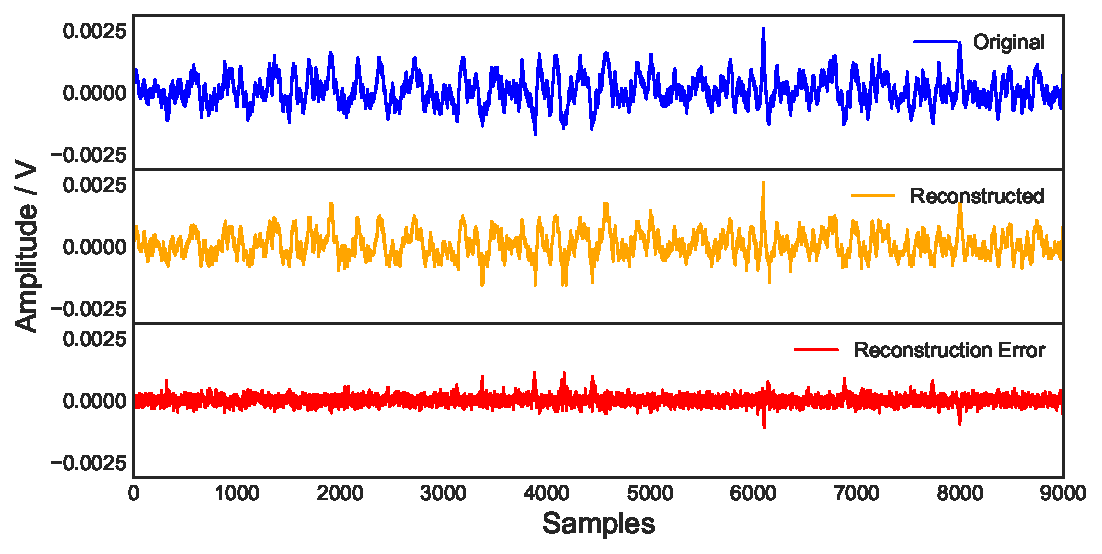
\includegraphics[width=1.0\textwidth]{fig/kmeans_large_4Vwater.pdf}
    \caption[K-means Large Motor Reconstruction In Water]{K-means reconstruction applied to three seconds of data from large motor running at 4V under a load applied through a fan and a bucket of water. Top: the original testing data. Middle: the reconstruction using K-means. Bottom: the reconstruction error between the reconstructed and original signal.}
    \label{fig:kmeans_large4Vwater}
\end{figure}

The presence of a load puts a large amount of stress on the motor. As the motor struggles to reach the desired voltage, a greater current is drawn, which leads to overheating.
        
There are many ways of adding a load to a motor, but attaching a fan immersed in water was chosen due to the ability to vary the load through using fans of different widths (1 cm, 2 cm and 3 cm).
    
Initially the test was done on a 12 V geared motor. A gear ratio of ${5}/{288}$ was found by counting the teeth of each cog and finding the speed of the connecting cog. This meant that the speed of the shaft, $\omega_1$, rotates at a much slower speed than the axle, $\omega _1$ as shown in Equation.~\eqref{eq:gear_Ratio}.

\begin{equation}
\omega_1 = \frac{5}{288} \omega_2.
\label{eq:gear_Ratio}
\end{equation}

This increases the torque of the shaft and resulted in the motor being able to deal with a greater load. It was even able to run at 30 V for the thickest fan.

A test was then conducted for another 12 V motor, this time ungeared. This time the motor could only reach a maximum of 4 V when the 1 cm fan was in use. This is evidence that as a load is added, a greater current is required to achieve a power that is large enough. A 10 A power supply was used for this experiment and this was the limiting factor, preventing the voltage from increasing further.

\subsection{Rotor Imbalance}
As the rotor spins within the motor, it is important for the weight to be evenly distributed around the central axle. Any imbalance present can cause the rotor to shift in position toward the areas of concentrated mass. As a motor runs increased levels of vibrations are produced with the frequency of the vibrations matching the shaft rotation speed. This unnecessarily increases the stress on the bearings and, in extreme cases, this can cause contact between the rotor and the stator. This increased strain on the bearings causes a larger friction, not only reducing the efficiency of the motor but also damaging the bearings. This can lead to complicated maintenance operations that would be otherwise unnecessary for a properly aligned motor.

If there is contact between the rotor and stator, there is again an increase in friction. This is often a larger frictional force, decreasing the efficiency further, but also generating large amounts of heat. When operated in this condition for long periods of time, this can cause overheating discussed above. As the rotor spins against the stator, the friction is capable of causing unwanted damage to both the rotor and the stator. In the case that this force is large enough, the permanent magnets could become detached from the stator, ultimately resulting in a failed motor.

Some possible causes of an imbalanced motor include uneven wear through use, design or assembly errors, and an eccentricity of the rotor or any physical damage distorting components. Observing additional, unexpected frequencies could be due to an imbalance within the motor, and as such are a warning sign to the decline in health of the motor. 

\begin{figure}
    \centering
    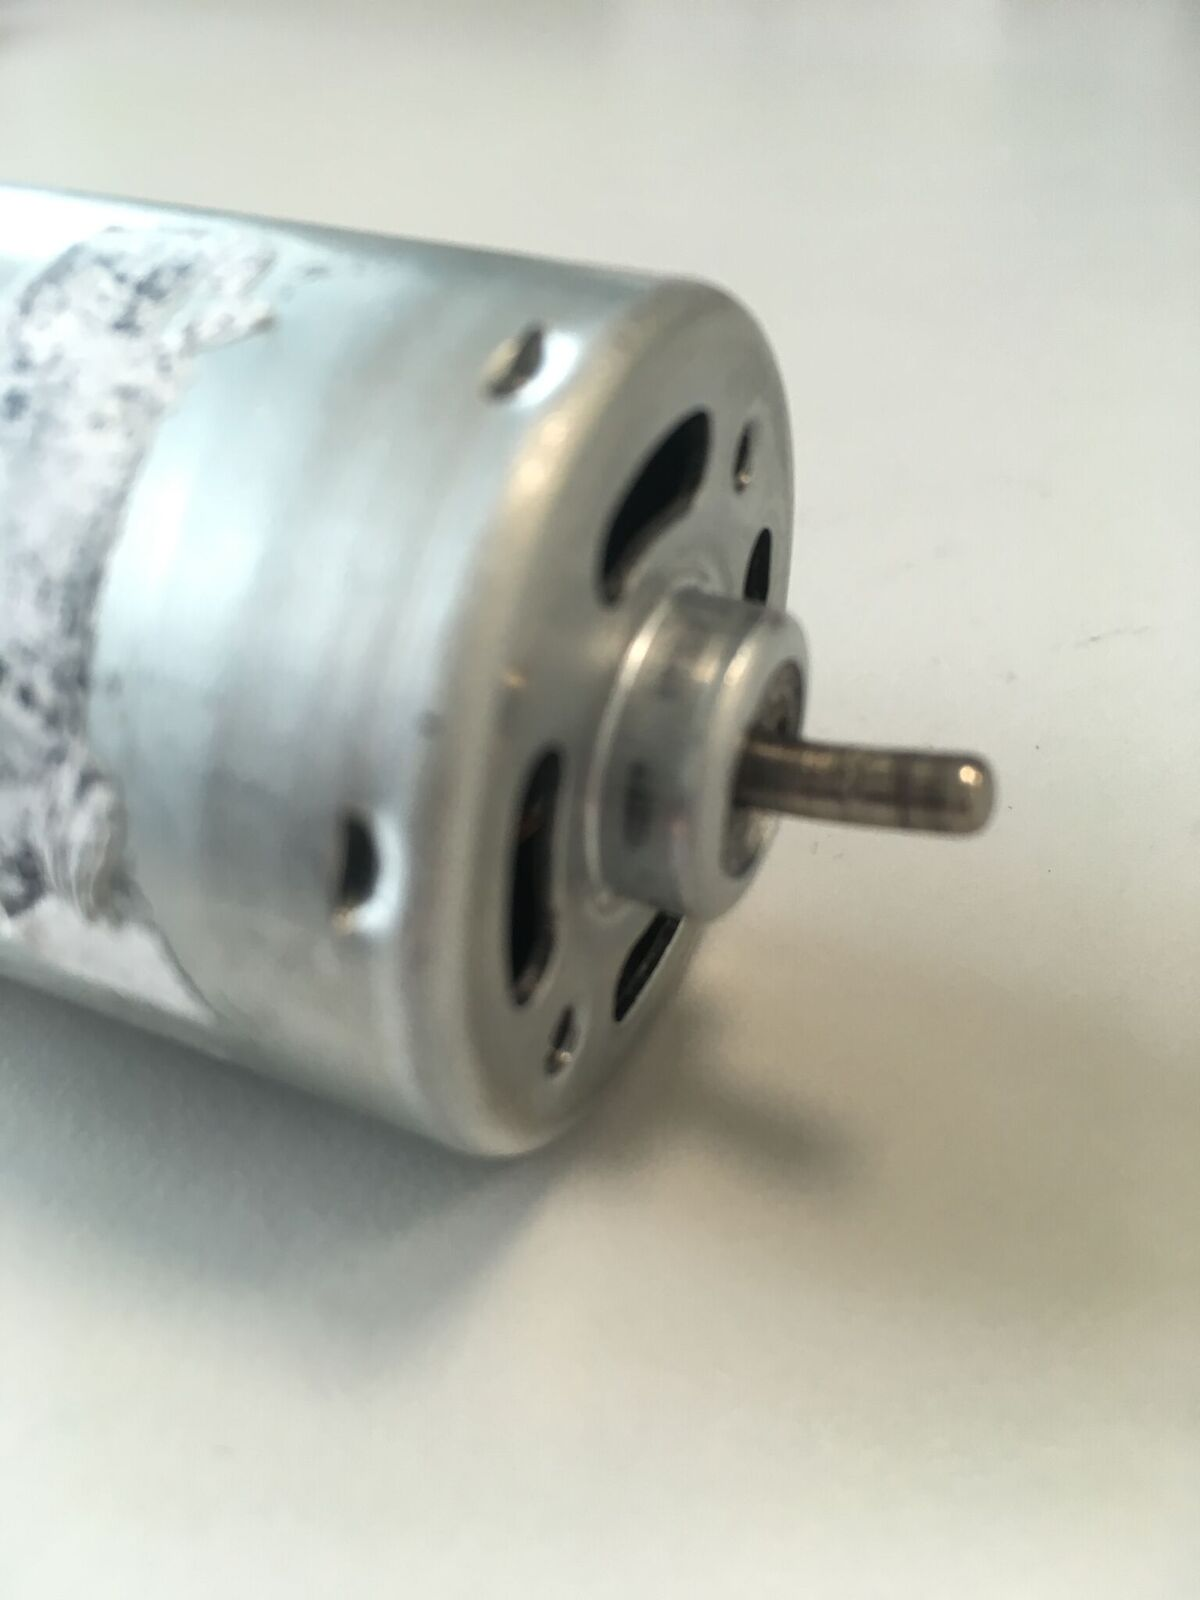
\includegraphics[trim={0cm, 15cm, 0cm, 8cm}, clip, width=0.5\textwidth]{bentshaft1.jpg}
    \caption[Misaligned Motor Shaft]{Small motor with misaligned shaft}
    \label{fig:bentshaft}
\end{figure}

To simulate an imbalanced motor, the shaft of a motor was bent with varying severities. (See Figure.~\ref{fig:bentshaft}.) As with all motors, it is impossible to attain a state of perfect balance, so small bends are expected in any initial baseline test. As the angle of the shaft from the normal was increased, the motors health deteriorated greatly. At large bends, the frictional force became so large that the motor required an initial force to start movement. This could represent a heavy contact between the rotor and the stator. 

%Normally, unbalance will produce a 1x or shaft speed vibration that is 80 percent or more of the total vibration. If 1x vibration is less than 80 percent, suspect other problems in addition to the unbalance.

\subsection{Brush Damage}
The brushes of a DC motor are a vital component, key to the proper working of the motor, allowing a DC power supply to provide an almost constant driving force throughout the entire revolution of the motor. The stationary brushes, combined with the rotating commutator attached to the rotor, periodically inverts the power supply throughout the revolutions. The commutator is composed of strips of conducting metal, usually copper, placed around the rotor. The strips of copper supply the current from the spring loaded brushes to the windings.  Without this periodic inversion of current direction through the windings, the motor would fail to spin and, as such, a good contact between the face of the brush and the commutator is necessary. 

The main cause of damage to the brushes of a DC motor usually occurs during maintenance. The soft surfaces of the carbon brushes can be easily scratched if not handled correctly. It is also possible that dirt can enter the motor housing during operation, which if found between the brush and the commutator, can cause heavy damage. In order to induce this type of failure mode, the brushes were treated with a heavy grit sandpaper, leaving the surface very rough. (picture of rough brushes here). 

It is possible for any imperfections in the surface of the carbon brushes to be removed without intervention during normal operation. As the rotor spins making contact with the face of the brushes, the friction generated is often capable of reducing the magnitude of the scratches. The possibility of this self repair will be investigated. However this friction of the brushes can cause another failure mode, loss of contact due to reduction in size of the brushes over time. This requires the brushes to be entirely replaced, making brushed motors unsuitable for use in remote locations. %more about self repair, what we did, e.g. left running for x volts for y time, more photos

The rough contact between the brush and commutator when damaged can cause sparking, leading to damaged commutators. Replacing the brush on a motor is a relatively simple maintenance task, however replacing the copper strips of a commutator can be more complicated. It is therefore important to ensure that a motor running with damaged brushes is identified immediately, to prevent running in sub-optimal conditions, potentially causing further damage. (picture here of commutator on small 12 V motor, this motor has copper strips for brushes, not carbon, so famously “sparky”)

Due to the flaws in the brushed DC motor model, their use has been declining with the introduction of brushless DC motors. These use an integrated switching power supply, to convert the DC to AC for the motor to run. Another alternative is to simply use an AC motor. 

\subsection{Gear Damage}

%First degreased the gears with a citrus degreasing spray.
%Added dirt to cause gears to break and prevent easy movement.
    %This can lead to overheating
%Placed in water for a few days to cause the motor to rust

\subsection{Specific Failures}

For testing purposed, to ensure that the various anomaly detection algorithms performed as expected, specific anomalies were induced. These included applying a force on the shaft, a routine of taps on the sensors or increasing and decreasing the voltage. The variations in frequencies induced by these actions are not found in a normal working motor, so the algorithm should detect these changes as anomalous. 

\subsection{Soft footing}

A motor running with soft footing can be the cause of multiple failures within a motor. When a motor with a misaligned shaft is coupled with an uneven motor housing, the uneven weight distribution as the rotor spins is exaggerated. The negative impacts of the uneven shaft are amplified, meaning even misalignments can now be damaging. 

The cause of a soft footing can be either an imperfection in the mounting feet of the motor, or the foundations the motor is mounted upon. In either case the motor will have the ability to move in a diagonal plane, similar to a chair or table on uneven ground, causing the shaft to become misaligned. This can be avoided by properly aligning the mountings and the foundations, commonly performed in industry using laser precision tools. 

This failure mode was induced by suspending the large motor above the work surface with a loosely gripped clamp stand. Any movement within the motor could cause a much larger movement in the stand, allowing the motor to oscillate while being suspended in the air. This oscillation will have an impact upon the shaft within the motor, exaggerating movements within the stator. The effects of this are similar to misalignment discussed above. Depending on the frequency of rotation of the motor, a resonance can occur, massively amplifying the oscillations causing an increased level of damage. If the feet do become loose, it is important to be aware of this before long term running of the motor is performed, as this would cause damage to internal components. It is more cost and energy effective to ensure proper footings prior to running.